% Generated by experiments/icpc/make_result_figs.py from committed results. Do not edit by hand.
\documentclass[border=2pt]{standalone}
\usepackage{pgfplots}\pgfplotsset{compat=1.18}
\usepackage{amsmath}
\definecolor{cblue}{HTML}{0072B2}\definecolor{cver}{HTML}{D55E00}\definecolor{cora}{HTML}{E69F00}
\definecolor{cgreen}{HTML}{009E73}\definecolor{cgrey}{HTML}{999999}\definecolor{csky}{HTML}{56B4E9}
\pgfplotsset{every axis/.append style={font=\footnotesize, tick label style={font=\scriptsize},
  label style={font=\footnotesize}, legend style={font=\scriptsize, draw=none, fill=none},
  axis lines*=left, ymajorgrids, grid style={black!8}}}
\begin{document}
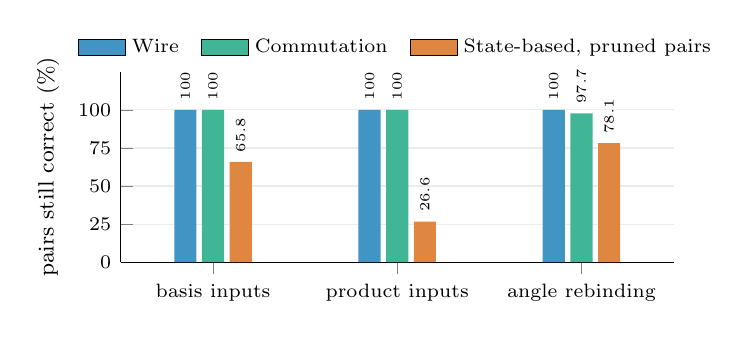
\begin{tikzpicture}\begin{axis}[ybar, bar width=8pt, width=8.6cm, height=4.0cm, ymin=0, ymax=125,
 ytick={0,25,50,75,100}, ylabel={pairs still correct (\%)}, symbolic x coords={basis inputs,product inputs,angle rebinding},
 xtick=data, enlarge x limits=0.25, nodes near coords, every node near coord/.append style={font=\tiny, rotate=90, anchor=west},
 nodes near coords={\pgfmathprintnumber[fixed,precision=1]{\pgfplotspointmeta}},
 legend style={at={(0.5,1.02)}, anchor=south, legend columns=3, /tikz/every even column/.append style={column sep=6pt}}, area legend]
\addplot[fill=cblue!75, draw=none] coordinates {(basis inputs,100.0) (product inputs,100.0) (angle rebinding,100.0)};
\addplot[fill=cgreen!75, draw=none] coordinates {(basis inputs,100.0) (product inputs,100.0) (angle rebinding,97.7)};
\addplot[fill=cver!75, draw=none] coordinates {(basis inputs,65.8) (product inputs,26.6) (angle rebinding,78.1)};
\legend{{Wire},{Commutation},{State-based, pruned pairs}}
\end{axis}\end{tikzpicture}
\end{document}
